% vim: set spell : spelllang=en_gb
\title{\bf Dynamic priority broadcasting channels:\\
	a multi-objective planning problem}
\author{Chiel Kooijman - 5743028\\University of Amsterdam}
\documentclass{article}
\usepackage{graphicx,amsmath}
\usepackage[round]{natbib}
\usepackage{multicol}
\usepackage{caption}
\def\keywords{\vspace{.5em}
	{\textbf{Keywords}:\,\relax
}}
\def\endkeywords{\par}
\newenvironment{tablehere}
{\def\@captype{table}}
{}

\newenvironment{figurehere}
{\def\@captype{figure}}
{}

\date{}
\setlength{\textwidth}{6.5in}
\setlength{\oddsidemargin}{0in}
\setlength{\evensidemargin}{0in}
\thispagestyle{empty}
\begin{document}
	\maketitle
	\begin{keywords}
		Dynamic Programming, MDP, Markov Decision Process, Multiobjective,
		Planning, Broadcasting Channel, Dynamic Priority
	\end{keywords}


	\begin{multicols}{2}

	\section{Introduction}
	\label{sec:introduction}
	In this research we extend the broadcasting channel problem as defined by
	\citet{ooi1996decentralized}, in order to account for situations in which
	multiple objectives are important, such as workload distribution in a data
	environment, distribution of traffic, or prioritisation of more important
	messages, in addition to throughput.
	In section \ref{sec:problem_definition} we redefine the problem to account
	for these considerations. Section \ref{sec:approach} covers the methods used
	to meet these requirements.
	% section introduction (end)

	\section{Problem definition}
	\label{sec:problem_definition}
	Multiple agents broadcast messages over a single channel, but only one
	message can be sent at any time, otherwise conflicts will arise and no
	message will come through. After a message is sent, the agents will know
	whether a message was sent, a conflict has arisen, or no message was sent.
	Agents have a single buffer that may contain a message.

	At any concrete time-step an agent $i$ with an empty buffer may get a new
	message with probability $p_i(s' |s, \vec{a})$ in a fully observable Markov
	decision process (MDP), and $p_i(s' \vec{o}|s, \vec{a})$ in a partially
	observable Markov decision process (POMDP) \citep{hansen2004dynamic}.

	The problem of optimising throughput has been solved for POMDPs
	\citep{ooi1996decentralized, hansen2004dynamic}, but in this case we would
	also like to avoid dominance of a single agent over the channel.

	Finding an optimal policy in terms of both throughput and dominance will
	first be solved for a fully observable MDP with two agents. Then the aim is
	to generalise towards any number of agents, a POMDP, and/or \emph{learning}
	the policy, dependent on the amount of time available.

	\citet{hansen2004dynamic} have given a solution with dynamic programming.
	This method will be extended so that for any weight vector $\vec{w}$ it will
	return the optimal Pareto-optimal set of solutions $\vec{w} \cdot
	\vec{V}^\pi$ \citep{vamplew2011empirical}, in a reward representation that
	can dynamically adapt priorities by changing the weights
	\citep{barrett2008learning,natarajan2005dynamic}.
	Equation \ref{eq:pareto} shows the definition for the Pareto-optimal set.
	\begin{equation}
		\label{eq:pareto}
		\Big\{ V\, \Big| \, \forall V'[ V \neq V' \land \exists n [V_n > V'_n]] \Big\}
	\end{equation}
	An example of a Pareto-optimal set for a two-dimensional system is shown in
	figure \ref{fig:pareto}.

	\begin{figurehere}
		\centering
		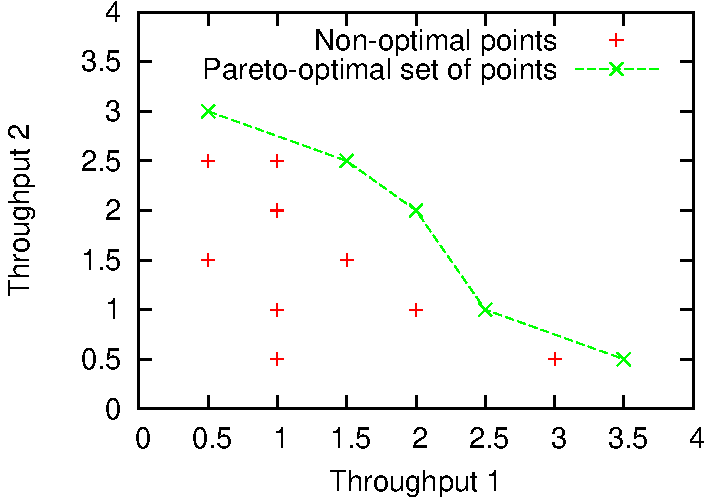
\includegraphics[scale=0.68]{images/pareto}
		\captionof{figure}{Pareto-optimal set in a two-dimensional system}
	   \label{fig:pareto}
	\end{figurehere}

	% section problem_definition (end)

	\section{Approach}
	\label{sec:approach}

		\subsection{Reward Representation}
		\label{sub:reward_representation}
		There are several ways to represent throughput and dominance in a vector.
		One approach is to have a two-dimensional vector $\vec{r}$ that contains
		the total throughput and some measure of dominance, for instance entropy
		or variance. An advantage of this approach is that the size of the reward
		vector is independent of the number of agents.

		Another way is to represent the vector as an $n$-dimensional vector:
		$$\vec{r} = \begin{bmatrix}
			t_1\\
			\vdots\\
			t_n\\
		\end{bmatrix}$$
		where $n$ is the number of agents, and each value represents the
		throughput of the corresponding agent. An advantage is that the vector
		contains more information than in the aforementioned representation, but
		there are many more states when the number of agents increases. It does
		however allow for prioritising messages (by changing the one of the
		weights), and the number of states can be greatly reduced, because every
		vector is equal to all of its permutations (provided we reorder the state
		vector and the reward vector in the same way).
		For example in a two-agent system, a state with a reward vector $\vec{r}$
		and function parameter $\vec{\theta}$
		vectors
		$$ f_{\vec{\theta}}(\vec{r})~\textrm{with}~\vec{r} = \begin{bmatrix}
			7\\
			3\\
		\end{bmatrix},~
		\vec{\theta} = \begin{bmatrix}
			w_1\\
			w_2\\
		\end{bmatrix}$$
		the value is equal to that of
		$$ f_{\vec{\theta}}(\vec{r})~\textrm{with}~\vec{r} = \begin{bmatrix}
			3\\
			7\\
		\end{bmatrix},~
		\vec{\theta} = \begin{bmatrix}
			w_2\\
			w_1\\
		\end{bmatrix}$$
		because all agents are equal and connected to the network in the same
		way.

		For these reasons the second representation was chosen.
		% subsection reward_representation (end)
	% section approach (end)
	\end{multicols}


	\section{Planning}
	\label{sec:planning}
	Find and read additional literature on the subject.\\
	Choose the representation and design an algorithm and describe optimisations
	etc.\\
	Implement the system in \texttt{C++} so that it may be extended with the
	MADP toolbox.
	% section planning (end)
	\pagebreak

	\bibliographystyle{plainnat}
	\bibliography{references}
\end{document}

